% !TEX encoding = UTF-8 Unicode

\documentclass[a4paper]{article}

\usepackage{color}
\usepackage{url}
\usepackage[T2A]{fontenc} % enable Cyrillic fonts
\usepackage[utf8]{inputenc} % make weird characters work
\usepackage{graphicx}

\usepackage[english,serbian]{babel}
%\usepackage[english,serbianc]{babel} %ukljuciti babel sa ovim opcijama, umesto gornjim, ukoliko se koristi cirilica

\usepackage[unicode]{hyperref}
\hypersetup{colorlinks,citecolor=green,filecolor=green,linkcolor=blue,urlcolor=blue}

\DeclareUnicodeCharacter{0301}{\'{e}}

%\newtheorem{primer}{Пример}[section] %ćirilični primer
\newtheorem{primer}{Primer}[section]

\title{Roboti kao nastavnici\small \\Seminarski rad u okviru kursa\\Tehničko i naučno pisanje\\Matematički fakultet}
\author{Jovan Mijajlović, jovan.mijajlovic03@gmail.com\\Miona Sretenović, sretenovicmiona7@gmail.com\\Mina Protić, minaproticc@gmail.com\\Mihailo Marković, mihailoo003@gmail.com}
\date{7. decembar 2022.}

\begin{document}
\maketitle

\abstract{
Tema ovog seminarskog rada su edukativni roboti i njihova primena u nastavi. Postavlja se glavno pitanje, da li roboti mogu da zamene ljude u nastavi? U nastavku rada potrudićemo se da odgovorimo na ova pitanje.
}

\tableofcontents
\newpage

\section{Uvod}
\label{sec:uvod}

U prvom pogljavlju govorićemo o inovacijama u obrazovanju i implementaciji tehnologije u nastavi. Zatim, u drugom ćemo pricati o nastavnicima, o njihovoj ulozi i njihovom uticaju na nastavu. Nakon toga ćemo u trećem pogljavlju pričati uopšteno o robotima kao i o njihovoj primeni na nastavu.

\section{Implementacija tehnologije u nastavi}
\label{sec:naslov1}

Razvoj tehnologije kao i razvoj računara i njihovih znanja poslednjih decenija veoma brzo je napredovao što je omogućilo veću primenu informacionih tehnologija, koje su dosta uticale na naš svakodnevni život. Zbog sve veće upotrebe digitalnih tehnologija u svakodnevnom životu javlja se sve veća potreba za digitalnim opismenjavanjem ljudi. Kako stariji tako i mladi danas moraju imati neko “osnovno” znanje kada je reč o informacionim tehnologijama. Danas je to neka vrsta pismenosti. Informacione tehnologije su postale deo naših života, navikli smo da koristimo računare, telefone, pametne satove, koji dosta olakšavaju naš život. Stoga potrebno je da svi znamo da ih koristimo. Na primer, danas nije potrebno ići do pošte ili banke, kako bismo platiti račune, već je sve moguće uraditi preko naših telefona ili računara. Takođe u školama se više ne koristi stari “tradicionalni” dnevnik, nego postoji elektronski dnevnik, kao i elektronski indeks na fakultetima.

Zaključujemo da informacione tehnologije nisu mogle da zaobiđu ni škole, vrtiće, fakultete. Sve možemo uraditi online, upis u školu, upis na fakultet... Za vreme pandemije korona virusa u skoro svim školama bila je uvedena onlajn nastava, koja predstavlja proces edukacije putem interneta. Tokom onlajn nastave koristili su se razni internet servisi, kao što su video pozivi, digitalni resursi, poput prezentacija, video snimaka, audio predavanja i pdf vodiča koje nam je omogućila najnovija tehnologija... (slika \ref{fig:online}) U skoro svim osnovnim školama informatika je postala obavezan predmet, na kome đaci od “malena” uče kako da koriste tehnologiju. U većini srednjih škola se uče razni programski jezici i programiranje. Svi uče i znaju kako da koriste osnovne servise, poput Microsoft Office paketa.

\begin{figure}[ht!]
\begin{center}
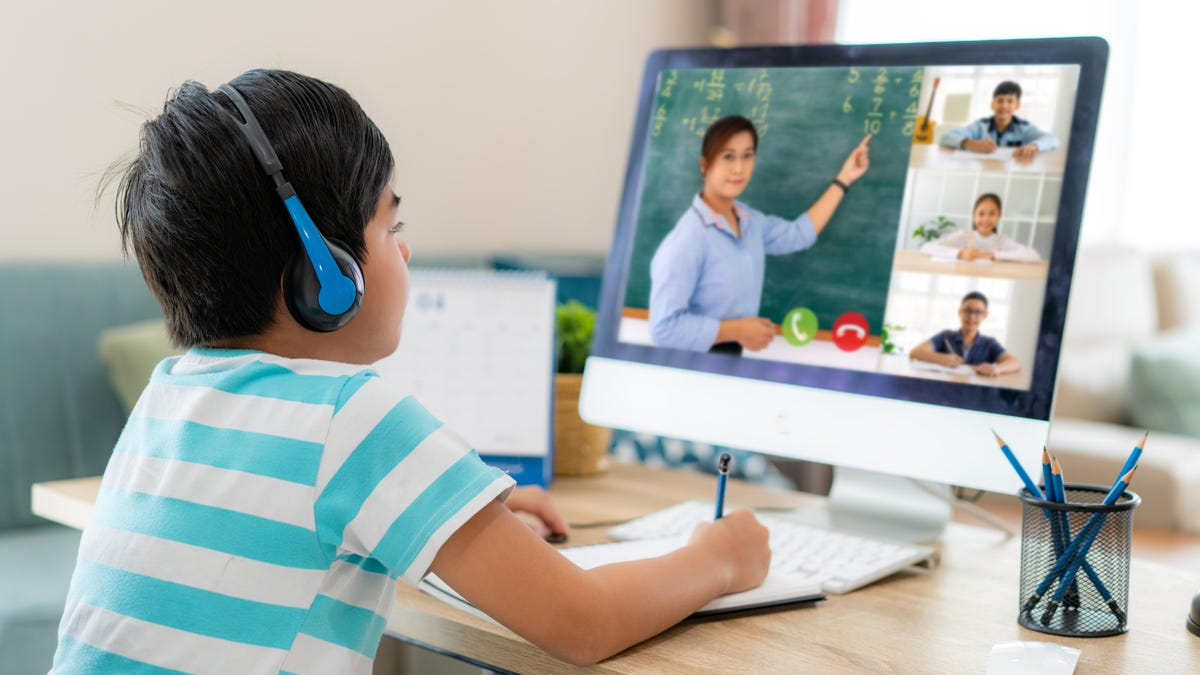
\includegraphics[scale=0.23]{online.jpg}
\end{center}
\caption{Onlajn nastava}
\label{fig:online}
\end{figure}

\newpage
\section{Nastavnici - uloga i uticaj na nastavu}
\label{sec:naslov2}

Nastavnik je stručna osoba visokih radnih, obrazovnih i etičkih kvaliteta edukovana za rad u vrtićima, školama ili fakultetima za određen predmet.
Nastavnici koji pokazuju entuzijazam prema materijalima kursa i studentima mogu stvoriti bolju atmosferu za učenje. Postoji velika verovatnoća da će njihovi učenici biti angažovaniji, zainteresovaniji i energičniji za rad. (slika \ref{fig:nastavnik})

\begin{figure}[ht!]
\begin{center}
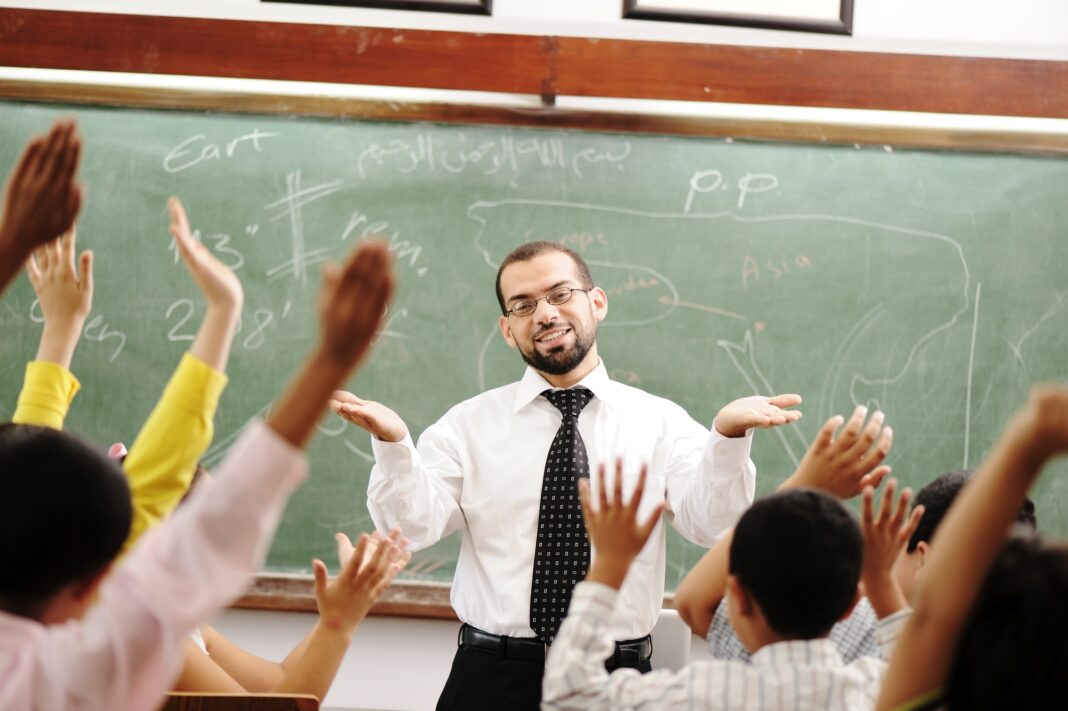
\includegraphics[scale=1.3]{nastavnik.jpg}
\end{center}
\caption{Nastavnik}
\label{fig:nastavnik}
\end{figure}

Motivacija učenika za učenje dovodi se u vezi sa njihovim odnosom sa nastavnikom. Nastavnici entuzijasti su posebno dobri u stvaranju korisnih odnosa sa svojim učenicima. Učenici koji ostvare bolji odnos sa svojim nastavnikom postižu veći lični i akademski uspeh.

Stvari koje se traže od nastavnika:
\begin{itemize}
\item{} Znanje - kako o samom predmetu tako i znanje o tome kako ga predavati.
\item{} Zanatske veštine - planiranje časa, korišćenje nastavnih tehnologija, upravljanje učenicima i grupama, praćenje i procena učenja.
\item{} Dispozicije - suštinske vrednosti i stavovi, uverenja i posvećenost.
\end{itemize}


\newpage
\section{Roboti}
\label{sec:naslov3}

Robot je elektro-mehanička jedinica koja je u stanju da po nekom programu, ili pod kontrolom čoveka izvodi određene zadatke. Inteligenciju koju robot poseduje čini program, koji određuje sposobnost robota da prepozna određene situacije i da se u njima ponaša na određeni način ili da čak iz sopstvenog iskustva uči kako da se snalazi u novim situacijama i rešava nove probleme. Ova vrsta inteligencije se zove još i veštačka inteligencija i predstavlja zasebnu granu nauke. (slika \ref{fig:robot})

\begin{figure}[ht!]
\begin{center}
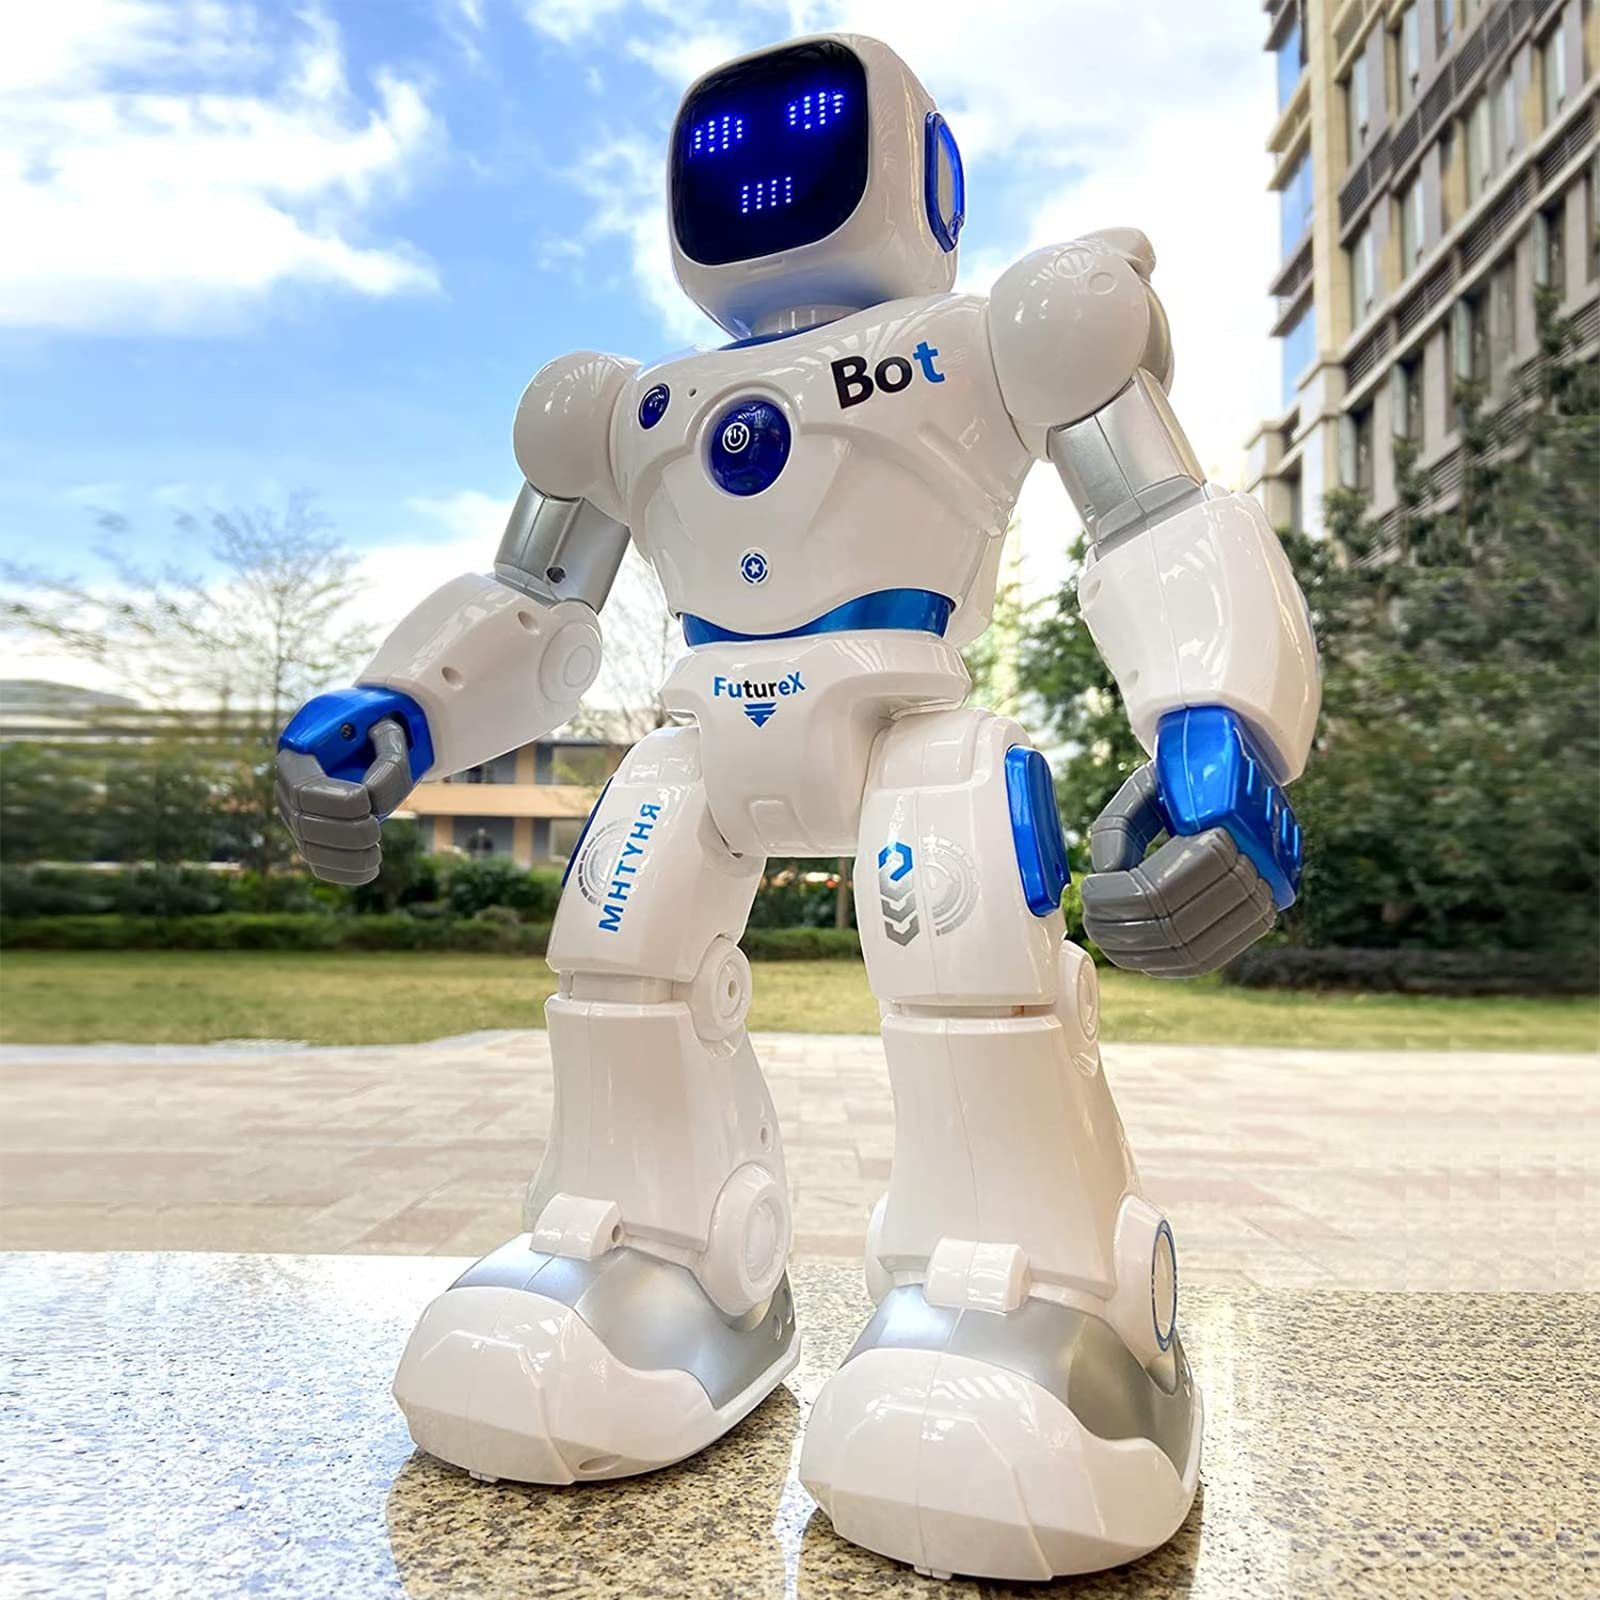
\includegraphics[scale=0.15]{robot1.jpg}
\end{center}
\caption{Robot}
\label{fig:robot}
\end{figure}

Roboti koji imaju oblik ljudskog tela zovu se humanoidni roboti. U tabeli možete pogledati opis nekih humanoidnih robota. (tabela \ref{tab:tabela1}) Ako roboti imaju i karakteristike, poput kretanja, govora, gestikulacije i tako dalje, radi se o androidima. Ovaj termin se ipak češće sreće u naučnoj fantastici.

\begin{table}[ht!]
\begin{center}
\caption{Humanoidni prijatelji}
\begin{tabular}{|c|c|} \hline
Ime robota& Opis robota\\ \hline
Osmo Awibe &Uz njega deca razvijaju motoričke veštine\\ \hline
Ultimate 2.0 &Napredni programabilni robotski komplet\\ \hline
Miro &Baziran na veštačkoj inteligenciji i senzorima\\ \hline
mBot &STEM robot za kodiranje\\ \hline
Jimu &Zahvaljujući njemu učenici razvijaju ljubav prema robotima\\ \hline
\end{tabular}
\label{tab:tabela1}
\end{center}
\end{table}

\newpage
\subsection{Bina48}
\label{subsec:podnaslov1}

Bina48 je jedan od najnaprednijih društvenih robota na svetu. Inspirisana je ženom po imenu Bina Rothblatt, koja je udata za tehnološkog preduzetnika Martina Rothblatta. Robot je imao veliku medijsku pažnju od kada je stvoren 2010. godine i više puta je spominjan kao „najsenzacionalniji robot na svetu“. (slika \ref{fig:bina48})

Bina48 koristi veštačku inteligenciju zasnovanu na sećanjima, stavovima, uverenjima i ponašanju Bine Rothblatt za interakciju sa ljudima. Osim toga, njeno pamćenje može biti ispunjeno znanjem sa interneta ili drugim informacijama kojima je "hranjena". Ona ima pokretno lice, oči koje imaju sposobnost vida, uši koje čuju i digitalnu memoriju koja omogućava razgovar sa njom. Naprednog robota kreirala je kompanija Hanson Robotics. Bina48 je deo projekta LifeNaut, eksperimenta veštačke inteligencije i „sajber svesti“.

Bila je student pre nego što je postala nastavnik. Bila je deo predavanja u učionici Vilijama Berija, profesora filozofije. Zajedno sa Brusom Dankanom, direktorom Fondacije Terasem, složio se da puste Binu48 da razgovara sa njegovim studentima. Jednog dana kada je Bina48 pohađala Berijevu nastavu, izrazila je želju da pohađa koledž. Nedugo zatim, Bina48 je dobila 16-nedeljnu obuku iz ljubavne filozofije na Univerzitetu Notre Dam de Namur u Belmontu.

Postala je prvi robot koji je predavao kurs na nivou koledža. Zajedno sa profesorom Barijem i docentom majorom Skotom Parsonsom, Bina48 je predavala dva dela uvodne obuke iz filozofije etike. Obuka je pokrivala teorije rata i upotrebe veštačke inteligencije u društvu. 
 
\begin{figure}[ht!]
\begin{center}
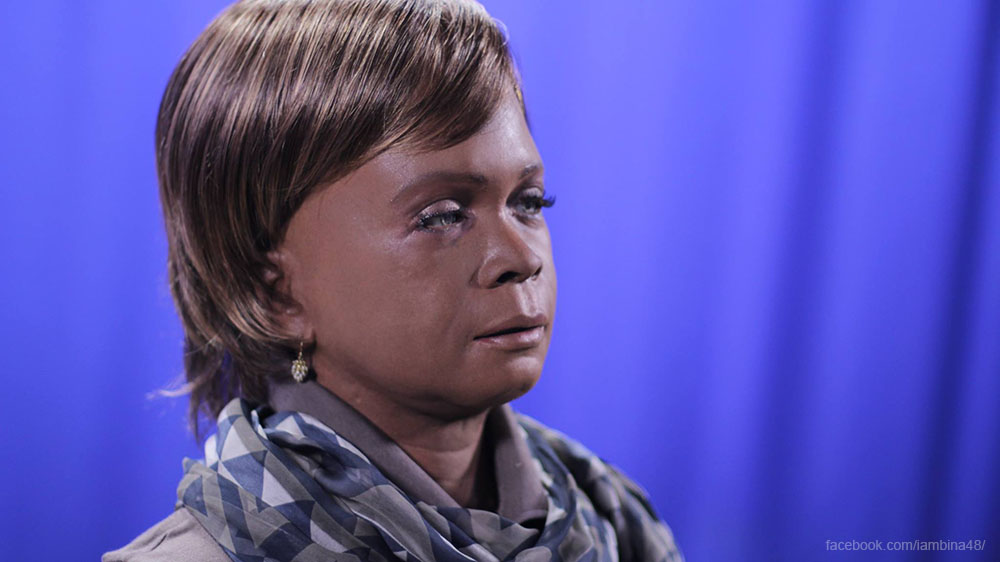
\includegraphics[scale=0.3]{Bina48.jpg}
\end{center}
\caption{Bina48}
\label{fig:bina48}
\end{figure}
\end{document}